\documentclass[1p]{elsarticle_modified}
%\bibliographystyle{elsarticle-num}

%\usepackage[colorlinks]{hyperref}
%\usepackage{abbrmath_seonhwa} %\Abb, \Ascr, \Acal ,\Abf, \Afrak
\usepackage{amsfonts}
\usepackage{amssymb}
\usepackage{amsmath}
\usepackage{amsthm}
\usepackage{scalefnt}
\usepackage{amsbsy}
\usepackage{kotex}
\usepackage{caption}
\usepackage{subfig}
\usepackage{color}
\usepackage{graphicx}
\usepackage{xcolor} %% white, black, red, green, blue, cyan, magenta, yellow
\usepackage{float}
\usepackage{setspace}
\usepackage{hyperref}

\usepackage{tikz}
\usetikzlibrary{arrows}

\usepackage{multirow}
\usepackage{array} % fixed length table
\usepackage{hhline}

%%%%%%%%%%%%%%%%%%%%%
\makeatletter
\renewcommand*\env@matrix[1][\arraystretch]{%
	\edef\arraystretch{#1}%
	\hskip -\arraycolsep
	\let\@ifnextchar\new@ifnextchar
	\array{*\c@MaxMatrixCols c}}
\makeatother %https://tex.stackexchange.com/questions/14071/how-can-i-increase-the-line-spacing-in-a-matrix
%%%%%%%%%%%%%%%

\usepackage[normalem]{ulem}

\newcommand{\msout}[1]{\ifmmode\text{\sout{\ensuremath{#1}}}\else\sout{#1}\fi}
%SOURCE: \msout is \stkout macro in https://tex.stackexchange.com/questions/20609/strikeout-in-math-mode

\newcommand{\cancel}[1]{
	\ifmmode
	{\color{red}\msout{#1}}
	\else
	{\color{red}\sout{#1}}
	\fi
}

\newcommand{\add}[1]{
	{\color{blue}\uwave{#1}}
}

\newcommand{\replace}[2]{
	\ifmmode
	{\color{red}\msout{#1}}{\color{blue}\uwave{#2}}
	\else
	{\color{red}\sout{#1}}{\color{blue}\uwave{#2}}
	\fi
}

\newcommand{\Sol}{\mathcal{S}} %segment
\newcommand{\D}{D} %diagram
\newcommand{\A}{\mathcal{A}} %arc


%%%%%%%%%%%%%%%%%%%%%%%%%%%%%5 test

\def\sl{\operatorname{\textup{SL}}(2,\Cbb)}
\def\psl{\operatorname{\textup{PSL}}(2,\Cbb)}
\def\quan{\mkern 1mu \triangleright \mkern 1mu}

\theoremstyle{definition}
\newtheorem{thm}{Theorem}[section]
\newtheorem{prop}[thm]{Proposition}
\newtheorem{lem}[thm]{Lemma}
\newtheorem{ques}[thm]{Question}
\newtheorem{cor}[thm]{Corollary}
\newtheorem{defn}[thm]{Definition}
\newtheorem{exam}[thm]{Example}
\newtheorem{rmk}[thm]{Remark}
\newtheorem{alg}[thm]{Algorithm}

\newcommand{\I}{\sqrt{-1}}
\begin{document}

%\begin{frontmatter}
%
%\title{Boundary parabolic representations of knots up to 8 crossings}
%
%%% Group authors per affiliation:
%\author{Yunhi Cho} 
%\address{Department of Mathematics, University of Seoul, Seoul, Korea}
%\ead{yhcho@uos.ac.kr}
%
%
%\author{Seonhwa Kim} %\fnref{s_kim}}
%\address{Center for Geometry and Physics, Institute for Basic Science, Pohang, 37673, Korea}
%\ead{ryeona17@ibs.re.kr}
%
%\author{Hyuk Kim}
%\address{Department of Mathematical Sciences, Seoul National University, Seoul 08826, Korea}
%\ead{hyukkim@snu.ac.kr}
%
%\author{Seokbeom Yoon}
%\address{Department of Mathematical Sciences, Seoul National University, Seoul, 08826,  Korea}
%\ead{sbyoon15@snu.ac.kr}
%
%\begin{abstract}
%We find all boundary parabolic representation of knots up to 8 crossings.
%
%\end{abstract}
%\begin{keyword}
%    \MSC[2010] 57M25 
%\end{keyword}
%
%\end{frontmatter}

%\linenumbers
%\tableofcontents
%
\newcommand\colored[1]{\textcolor{white}{\rule[-0.35ex]{0.8em}{1.4ex}}\kern-0.8em\color{red} #1}%
%\newcommand\colored[1]{\textcolor{white}{ #1}\kern-2.17ex	\textcolor{white}{ #1}\kern-1.81ex	\textcolor{white}{ #1}\kern-2.15ex\color{red}#1	}

{\Large $\underline{12n_{0719}~(K12n_{0719})}$}

\setlength{\tabcolsep}{10pt}
\renewcommand{\arraystretch}{1.6}
\vspace{1cm}\begin{tabular}{m{100pt}>{\centering\arraybackslash}m{274pt}}
\multirow{5}{120pt}{
	\centering
	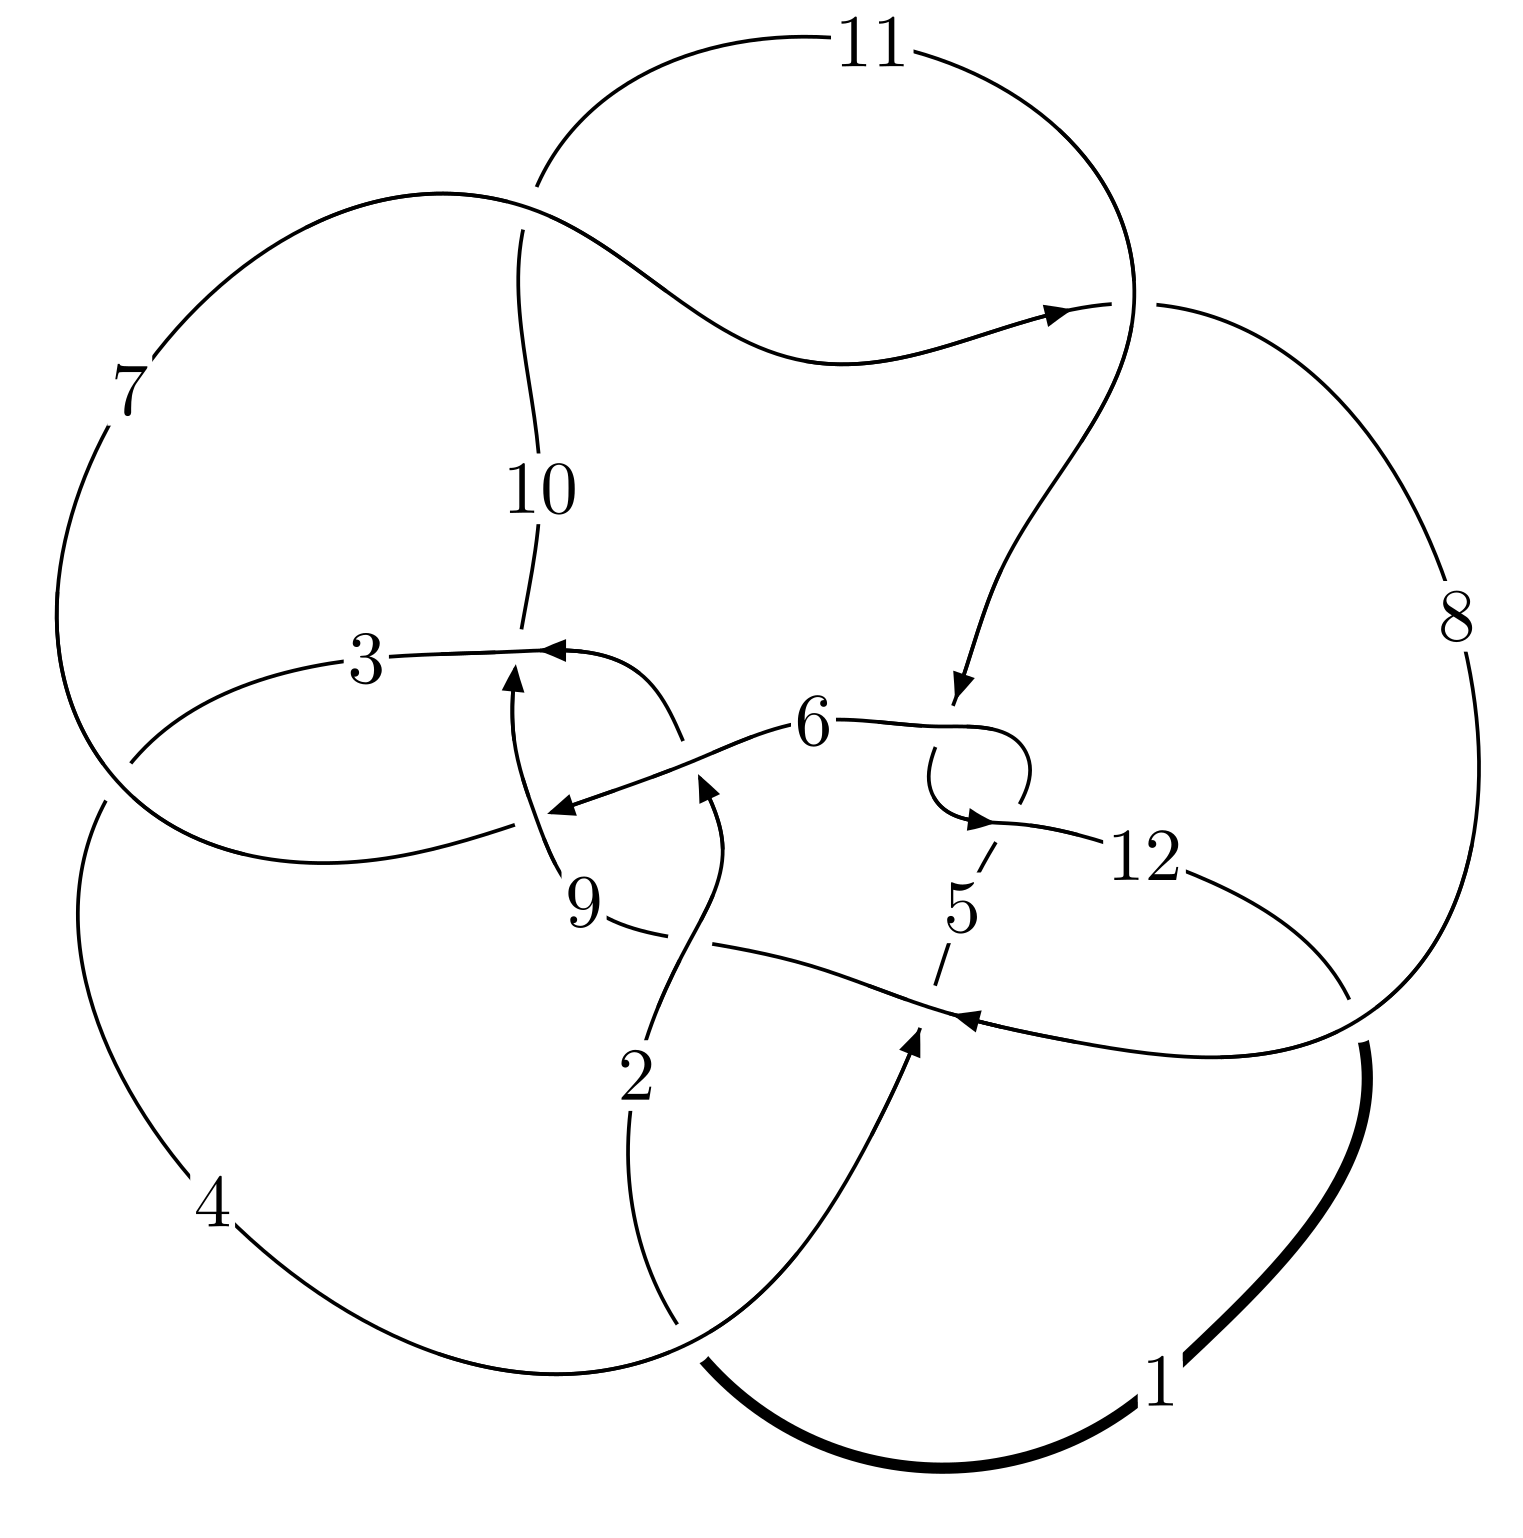
\includegraphics[width=112pt]{../../../GIT/diagram.site/Diagrams/png/2808_12n_0719.png}\\
\ \ \ A knot diagram\footnotemark}&
\allowdisplaybreaks
\textbf{Linearized knot diagam} \\
\cline{2-2}
 &
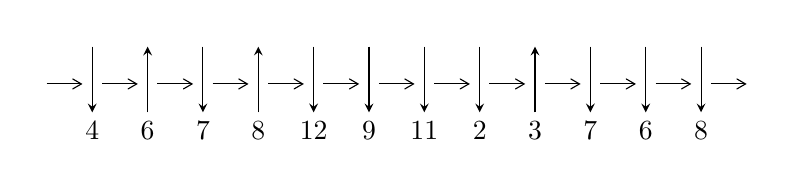
\begin{tikzpicture}[x=20pt, y=17pt]
	% nodes
	\node (C0) at (0, 0) {};
	\node (C1) at (1, 0) {};
	\node (C1U) at (1, +1) {};
	\node (C1D) at (1, -1) {4};

	\node (C2) at (2, 0) {};
	\node (C2U) at (2, +1) {};
	\node (C2D) at (2, -1) {6};

	\node (C3) at (3, 0) {};
	\node (C3U) at (3, +1) {};
	\node (C3D) at (3, -1) {7};

	\node (C4) at (4, 0) {};
	\node (C4U) at (4, +1) {};
	\node (C4D) at (4, -1) {8};

	\node (C5) at (5, 0) {};
	\node (C5U) at (5, +1) {};
	\node (C5D) at (5, -1) {12};

	\node (C6) at (6, 0) {};
	\node (C6U) at (6, +1) {};
	\node (C6D) at (6, -1) {9};

	\node (C7) at (7, 0) {};
	\node (C7U) at (7, +1) {};
	\node (C7D) at (7, -1) {11};

	\node (C8) at (8, 0) {};
	\node (C8U) at (8, +1) {};
	\node (C8D) at (8, -1) {2};

	\node (C9) at (9, 0) {};
	\node (C9U) at (9, +1) {};
	\node (C9D) at (9, -1) {3};

	\node (C10) at (10, 0) {};
	\node (C10U) at (10, +1) {};
	\node (C10D) at (10, -1) {7};

	\node (C11) at (11, 0) {};
	\node (C11U) at (11, +1) {};
	\node (C11D) at (11, -1) {6};

	\node (C12) at (12, 0) {};
	\node (C12U) at (12, +1) {};
	\node (C12D) at (12, -1) {8};
	\node (C13) at (13, 0) {};

	% arrows
	\draw[->,>={angle 60}]
	(C0) edge (C1) (C1) edge (C2) (C2) edge (C3) (C3) edge (C4) (C4) edge (C5) (C5) edge (C6) (C6) edge (C7) (C7) edge (C8) (C8) edge (C9) (C9) edge (C10) (C10) edge (C11) (C11) edge (C12) (C12) edge (C13) ;	\draw[->,>=stealth]
	(C1U) edge (C1D) (C2D) edge (C2U) (C3U) edge (C3D) (C4D) edge (C4U) (C5U) edge (C5D) (C6U) edge (C6D) (C7U) edge (C7D) (C8U) edge (C8D) (C9D) edge (C9U) (C10U) edge (C10D) (C11U) edge (C11D) (C12U) edge (C12D) ;
	\end{tikzpicture} \\
\hhline{~~} \\& 
\textbf{Solving Sequence} \\ \cline{2-2} 
 &
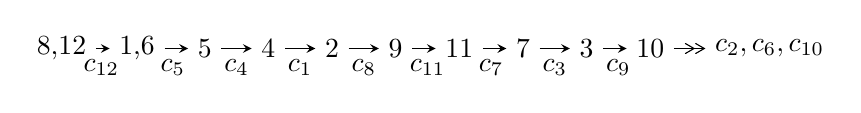
\begin{tikzpicture}[x=23pt, y=7pt]
	% node
	\node (A0) at (-1/8, 0) {8,12};
	\node (A1) at (17/16, 0) {1,6};
	\node (A2) at (17/8, 0) {5};
	\node (A3) at (25/8, 0) {4};
	\node (A4) at (33/8, 0) {2};
	\node (A5) at (41/8, 0) {9};
	\node (A6) at (49/8, 0) {11};
	\node (A7) at (57/8, 0) {7};
	\node (A8) at (65/8, 0) {3};
	\node (A9) at (73/8, 0) {10};
	\node (C1) at (1/2, -1) {$c_{12}$};
	\node (C2) at (13/8, -1) {$c_{5}$};
	\node (C3) at (21/8, -1) {$c_{4}$};
	\node (C4) at (29/8, -1) {$c_{1}$};
	\node (C5) at (37/8, -1) {$c_{8}$};
	\node (C6) at (45/8, -1) {$c_{11}$};
	\node (C7) at (53/8, -1) {$c_{7}$};
	\node (C8) at (61/8, -1) {$c_{3}$};
	\node (C9) at (69/8, -1) {$c_{9}$};
	\node (A10) at (11, 0) {$c_{2},c_{6},c_{10}$};

	% edge
	\draw[->,>=stealth]	
	(A0) edge (A1) (A1) edge (A2) (A2) edge (A3) (A3) edge (A4) (A4) edge (A5) (A5) edge (A6) (A6) edge (A7) (A7) edge (A8) (A8) edge (A9) ;
	\draw[->>,>={angle 60}]	
	(A9) edge (A10);
\end{tikzpicture} \\ 

\end{tabular} \\

\footnotetext{
The image of knot diagram is generated by the software ``\textbf{Draw programme}" developed by Andrew Bartholomew(\url{http://www.layer8.co.uk/maths/draw/index.htm\#Running-draw}), where we modified some parts for our purpose(\url{https://github.com/CATsTAILs/LinksPainter}).
}\phantom \\ \newline 
\centering \textbf{Ideals for irreducible components\footnotemark of $X_{\text{par}}$} 
 
\begin{align*}
I^u_{1}&=\langle 
-9.27341\times10^{166} u^{43}-4.43348\times10^{165} u^{42}+\cdots+8.47031\times10^{167} b+9.37901\times10^{167},\\
\phantom{I^u_{1}}&\phantom{= \langle  }-2.43777\times10^{167} u^{43}-6.35520\times10^{166} u^{42}+\cdots+8.47031\times10^{167} a-2.63451\times10^{168},\\
\phantom{I^u_{1}}&\phantom{= \langle  }u^{44}+39 u^{42}+\cdots-4 u-1\rangle \\
I^u_{2}&=\langle 
479931 u^{10}-2120739 u^9+\cdots+70976 b-1189615,\\
\phantom{I^u_{2}}&\phantom{= \langle  }-238887 u^{10}+992743 u^9+\cdots+35488 a+973491,\\
\phantom{I^u_{2}}&\phantom{= \langle  }u^{11}-4 u^{10}+6 u^9-24 u^8+41 u^7+18 u^6+16 u^5-28 u^4-73 u^3-45 u^2-11 u-1\rangle \\
I^u_{3}&=\langle 
-7 u^5-33 u^4-82 u^3-73 u^2+23 b-11 u-13,\;51 u^5+247 u^4+673 u^3+798 u^2+23 a+504 u+236,\\
\phantom{I^u_{3}}&\phantom{= \langle  }u^6+5 u^5+14 u^4+18 u^3+13 u^2+7 u+1\rangle \\
\\
\end{align*}
\raggedright * 3 irreducible components of $\dim_{\mathbb{C}}=0$, with total 61 representations.\\
\footnotetext{All coefficients of polynomials are rational numbers. But the coefficients are sometimes approximated in decimal forms when there is not enough margin.}
\newpage
\renewcommand{\arraystretch}{1}
\centering \section*{I. $I^u_{1}= \langle -9.27\times10^{166} u^{43}-4.43\times10^{165} u^{42}+\cdots+8.47\times10^{167} b+9.38\times10^{167},\;-2.44\times10^{167} u^{43}-6.36\times10^{166} u^{42}+\cdots+8.47\times10^{167} a-2.63\times10^{168},\;u^{44}+39 u^{42}+\cdots-4 u-1 \rangle$}
\flushleft \textbf{(i) Arc colorings}\\
\begin{tabular}{m{7pt} m{180pt} m{7pt} m{180pt} }
\flushright $a_{8}=$&$\begin{pmatrix}0\\u\end{pmatrix}$ \\
\flushright $a_{12}=$&$\begin{pmatrix}1\\0\end{pmatrix}$ \\
\flushright $a_{1}=$&$\begin{pmatrix}1\\u^2\end{pmatrix}$ \\
\flushright $a_{6}=$&$\begin{pmatrix}0.287802 u^{43}+0.0750292 u^{42}+\cdots-75.3078 u+3.11029\\0.109481 u^{43}+0.00523414 u^{42}+\cdots-7.77140 u-1.10728\end{pmatrix}$ \\
\flushright $a_{5}=$&$\begin{pmatrix}0.397283 u^{43}+0.0802633 u^{42}+\cdots-83.0792 u+2.00301\\0.109481 u^{43}+0.00523414 u^{42}+\cdots-7.77140 u-1.10728\end{pmatrix}$ \\
\flushright $a_{4}=$&$\begin{pmatrix}0.397283 u^{43}+0.0802633 u^{42}+\cdots-83.0792 u+2.00301\\0.0983593 u^{43}+0.00483973 u^{42}+\cdots-7.05306 u-1.02702\end{pmatrix}$ \\
\flushright $a_{2}=$&$\begin{pmatrix}-0.470002 u^{43}-0.00424396 u^{42}+\cdots+29.0832 u-7.19779\\-0.112085 u^{43}+0.000633314 u^{42}+\cdots+12.6945 u+0.279509\end{pmatrix}$ \\
\flushright $a_{9}=$&$\begin{pmatrix}0.102867 u^{43}+0.129659 u^{42}+\cdots-63.4031 u-16.1083\\-0.199965 u^{43}+0.0128457 u^{42}+\cdots+5.55859 u-0.338500\end{pmatrix}$ \\
\flushright $a_{11}=$&$\begin{pmatrix}0.333819 u^{43}+0.00512371 u^{42}+\cdots-15.9017 u+9.48154\\0.136183 u^{43}-0.000879747 u^{42}+\cdots-13.1815 u-0.283753\end{pmatrix}$ \\
\flushright $a_{7}=$&$\begin{pmatrix}-0.476846 u^{43}-0.199627 u^{42}+\cdots+108.229 u+16.5533\\0.192885 u^{43}-0.0142872 u^{42}+\cdots-0.0996084 u+0.694413\end{pmatrix}$ \\
\flushright $a_{3}=$&$\begin{pmatrix}-1.09702 u^{43}-0.168014 u^{42}+\cdots+172.835 u-5.26974\\-0.161947 u^{43}-0.00324765 u^{42}+\cdots+21.6795 u+2.19727\end{pmatrix}$ \\
\flushright $a_{10}=$&$\begin{pmatrix}-1.65580 u^{43}-0.222262 u^{42}+\cdots+263.566 u-14.2425\\-0.361239 u^{43}-0.00429338 u^{42}+\cdots+33.9954 u+3.61276\end{pmatrix}$\\&\end{tabular}
\flushleft \textbf{(ii) Obstruction class $= -1$}\\~\\
\flushleft \textbf{(iii) Cusp Shapes $= -0.617620 u^{43}-0.0398235 u^{42}+\cdots+49.7144 u-0.605176$}\\~\\
\newpage\renewcommand{\arraystretch}{1}
\flushleft \textbf{(iv) u-Polynomials at the component}\newline \\
\begin{tabular}{m{50pt}|m{274pt}}
Crossings & \hspace{64pt}u-Polynomials at each crossing \\
\hline $$\begin{aligned}c_{1},c_{5},c_{11}\end{aligned}$$&$\begin{aligned}
&u^{44}- u^{43}+\cdots-22 u-1
\end{aligned}$\\
\hline $$\begin{aligned}c_{2}\end{aligned}$$&$\begin{aligned}
&u^{44}-2 u^{43}+\cdots+544 u+64
\end{aligned}$\\
\hline $$\begin{aligned}c_{3}\end{aligned}$$&$\begin{aligned}
&u^{44}+2 u^{43}+\cdots+68 u-52
\end{aligned}$\\
\hline $$\begin{aligned}c_{4}\end{aligned}$$&$\begin{aligned}
&u^{44}-32 u^{42}+\cdots+6459 u+461
\end{aligned}$\\
\hline $$\begin{aligned}c_{6}\end{aligned}$$&$\begin{aligned}
&u^{44}-5 u^{42}+\cdots-11 u+1
\end{aligned}$\\
\hline $$\begin{aligned}c_{7},c_{10}\end{aligned}$$&$\begin{aligned}
&u^{44}+u^{43}+\cdots-108 u-11
\end{aligned}$\\
\hline $$\begin{aligned}c_{8}\end{aligned}$$&$\begin{aligned}
&u^{44}+u^{43}+\cdots-288 u+32
\end{aligned}$\\
\hline $$\begin{aligned}c_{9}\end{aligned}$$&$\begin{aligned}
&u^{44}- u^{43}+\cdots-46 u+43
\end{aligned}$\\
\hline $$\begin{aligned}c_{12}\end{aligned}$$&$\begin{aligned}
&u^{44}+39 u^{42}+\cdots+4 u-1
\end{aligned}$\\
\hline
\end{tabular}\\~\\
\newpage\renewcommand{\arraystretch}{1}
\flushleft \textbf{(v) Riley Polynomials at the component}\newline \\
\begin{tabular}{m{50pt}|m{274pt}}
Crossings & \hspace{64pt}Riley Polynomials at each crossing \\
\hline $$\begin{aligned}c_{1},c_{5},c_{11}\end{aligned}$$&$\begin{aligned}
&y^{44}+59 y^{43}+\cdots+50 y+1
\end{aligned}$\\
\hline $$\begin{aligned}c_{2}\end{aligned}$$&$\begin{aligned}
&y^{44}-26 y^{43}+\cdots-246784 y+4096
\end{aligned}$\\
\hline $$\begin{aligned}c_{3}\end{aligned}$$&$\begin{aligned}
&y^{44}+46 y^{43}+\cdots-55168 y+2704
\end{aligned}$\\
\hline $$\begin{aligned}c_{4}\end{aligned}$$&$\begin{aligned}
&y^{44}-64 y^{43}+\cdots-67584469 y+212521
\end{aligned}$\\
\hline $$\begin{aligned}c_{6}\end{aligned}$$&$\begin{aligned}
&y^{44}-10 y^{43}+\cdots-41 y+1
\end{aligned}$\\
\hline $$\begin{aligned}c_{7},c_{10}\end{aligned}$$&$\begin{aligned}
&y^{44}+7 y^{43}+\cdots+1822 y+121
\end{aligned}$\\
\hline $$\begin{aligned}c_{8}\end{aligned}$$&$\begin{aligned}
&y^{44}-3 y^{43}+\cdots-139264 y+1024
\end{aligned}$\\
\hline $$\begin{aligned}c_{9}\end{aligned}$$&$\begin{aligned}
&y^{44}-39 y^{43}+\cdots-62660 y+1849
\end{aligned}$\\
\hline $$\begin{aligned}c_{12}\end{aligned}$$&$\begin{aligned}
&y^{44}+78 y^{43}+\cdots+108 y+1
\end{aligned}$\\
\hline
\end{tabular}\\~\\
\newpage\flushleft \textbf{(vi) Complex Volumes and Cusp Shapes}
$$\begin{array}{c|c|c}  
\text{Solutions to }I^u_{1}& \I (\text{vol} + \sqrt{-1}CS) & \text{Cusp shape}\\
 \hline 
\begin{aligned}
u &= -0.653028 + 0.479211 I \\
a &= -0.78323 + 1.75591 I \\
b &= \phantom{-}0.0581394 - 0.0762256 I\end{aligned}
 & \phantom{-}0.33032 + 4.70980 I & -11.3107 - 11.5969 I \\ \hline\begin{aligned}
u &= -0.653028 - 0.479211 I \\
a &= -0.78323 - 1.75591 I \\
b &= \phantom{-}0.0581394 + 0.0762256 I\end{aligned}
 & \phantom{-}0.33032 - 4.70980 I & -11.3107 + 11.5969 I \\ \hline\begin{aligned}
u &= \phantom{-}0.027724 + 0.750161 I \\
a &= \phantom{-}0.567924 + 0.078651 I \\
b &= -0.974182 + 0.157306 I\end{aligned}
 & \phantom{-}3.27845 - 3.12920 I & -2.75319 + 2.59759 I \\ \hline\begin{aligned}
u &= \phantom{-}0.027724 - 0.750161 I \\
a &= \phantom{-}0.567924 - 0.078651 I \\
b &= -0.974182 - 0.157306 I\end{aligned}
 & \phantom{-}3.27845 + 3.12920 I & -2.75319 - 2.59759 I \\ \hline\begin{aligned}
u &= \phantom{-}0.670831 + 0.205742 I \\
a &= \phantom{-}0.836569 + 0.484990 I \\
b &= \phantom{-}0.185017 + 0.160225 I\end{aligned}
 & -1.208230 - 0.322851 I & -9.94677 + 2.27028 I \\ \hline\begin{aligned}
u &= \phantom{-}0.670831 - 0.205742 I \\
a &= \phantom{-}0.836569 - 0.484990 I \\
b &= \phantom{-}0.185017 - 0.160225 I\end{aligned}
 & -1.208230 + 0.322851 I & -9.94677 - 2.27028 I \\ \hline\begin{aligned}
u &= \phantom{-}1.31394\phantom{ +0.000000I} \\
a &= \phantom{-}0.393355\phantom{ +0.000000I} \\
b &= \phantom{-}0.433533\phantom{ +0.000000I}\end{aligned}
 & -2.58215\phantom{ +0.000000I} & \phantom{-0.000000 } 0 \\ \hline\begin{aligned}
u &= -1.31681\phantom{ +0.000000I} \\
a &= -0.520583\phantom{ +0.000000I} \\
b &= \phantom{-}0.478115\phantom{ +0.000000I}\end{aligned}
 & -6.41728\phantom{ +0.000000I} & \phantom{-0.000000 } 0 \\ \hline\begin{aligned}
u &= \phantom{-}0.021517 + 0.557538 I \\
a &= \phantom{-}1.282020 + 0.262721 I \\
b &= \phantom{-}0.233628 + 0.802395 I\end{aligned}
 & -0.05460 - 2.35319 I & -7.41013 + 4.71617 I \\ \hline\begin{aligned}
u &= \phantom{-}0.021517 - 0.557538 I \\
a &= \phantom{-}1.282020 - 0.262721 I \\
b &= \phantom{-}0.233628 - 0.802395 I\end{aligned}
 & -0.05460 + 2.35319 I & -7.41013 - 4.71617 I\\
 \hline 
 \end{array}$$\newpage$$\begin{array}{c|c|c}  
\text{Solutions to }I^u_{1}& \I (\text{vol} + \sqrt{-1}CS) & \text{Cusp shape}\\
 \hline 
\begin{aligned}
u &= -0.489487 + 0.154722 I \\
a &= \phantom{-}1.56149 - 0.49207 I \\
b &= \phantom{-}0.215149 + 0.758157 I\end{aligned}
 & \phantom{-}1.25902 - 2.03144 I & -0.14682 + 4.37003 I \\ \hline\begin{aligned}
u &= -0.489487 - 0.154722 I \\
a &= \phantom{-}1.56149 + 0.49207 I \\
b &= \phantom{-}0.215149 - 0.758157 I\end{aligned}
 & \phantom{-}1.25902 + 2.03144 I & -0.14682 - 4.37003 I \\ \hline\begin{aligned}
u &= \phantom{-}0.473973\phantom{ +0.000000I} \\
a &= \phantom{-}2.83673\phantom{ +0.000000I} \\
b &= -0.506626\phantom{ +0.000000I}\end{aligned}
 & -2.36937\phantom{ +0.000000I} & \phantom{-}1.94390\phantom{ +0.000000I} \\ \hline\begin{aligned}
u &= \phantom{-}0.460603\phantom{ +0.000000I} \\
a &= \phantom{-}1.26886\phantom{ +0.000000I} \\
b &= \phantom{-}0.519451\phantom{ +0.000000I}\end{aligned}
 & -1.16126\phantom{ +0.000000I} & -8.98030\phantom{ +0.000000I} \\ \hline\begin{aligned}
u &= \phantom{-}0.135939 + 0.415909 I \\
a &= -2.10897 - 1.43331 I \\
b &= \phantom{-}0.300845 + 1.228730 I\end{aligned}
 & -2.36079 - 2.76760 I & -10.42789 + 3.67232 I \\ \hline\begin{aligned}
u &= \phantom{-}0.135939 - 0.415909 I \\
a &= -2.10897 + 1.43331 I \\
b &= \phantom{-}0.300845 - 1.228730 I\end{aligned}
 & -2.36079 + 2.76760 I & -10.42789 - 3.67232 I \\ \hline\begin{aligned}
u &= -0.93702 + 1.28948 I \\
a &= -0.002221 - 0.962499 I \\
b &= \phantom{-}0.328930 + 1.368230 I\end{aligned}
 & \phantom{-}3.52831 - 3.02493 I & \phantom{-0.000000 } 0 \\ \hline\begin{aligned}
u &= -0.93702 - 1.28948 I \\
a &= -0.002221 + 0.962499 I \\
b &= \phantom{-}0.328930 - 1.368230 I\end{aligned}
 & \phantom{-}3.52831 + 3.02493 I & \phantom{-0.000000 } 0 \\ \hline\begin{aligned}
u &= -1.59462 + 0.32915 I \\
a &= -0.203262 + 0.245637 I \\
b &= -0.113423 - 1.192920 I\end{aligned}
 & \phantom{-}4.53063 + 4.34162 I & \phantom{-0.000000 } 0 \\ \hline\begin{aligned}
u &= -1.59462 - 0.32915 I \\
a &= -0.203262 - 0.245637 I \\
b &= -0.113423 + 1.192920 I\end{aligned}
 & \phantom{-}4.53063 - 4.34162 I & \phantom{-0.000000 } 0\\
 \hline 
 \end{array}$$\newpage$$\begin{array}{c|c|c}  
\text{Solutions to }I^u_{1}& \I (\text{vol} + \sqrt{-1}CS) & \text{Cusp shape}\\
 \hline 
\begin{aligned}
u &= \phantom{-}0.221192 + 0.259639 I \\
a &= \phantom{-}1.096330 - 0.751243 I \\
b &= \phantom{-}0.691688 + 0.860912 I\end{aligned}
 & -0.63985 - 2.51667 I & -0.25112 + 12.13395 I \\ \hline\begin{aligned}
u &= \phantom{-}0.221192 - 0.259639 I \\
a &= \phantom{-}1.096330 + 0.751243 I \\
b &= \phantom{-}0.691688 - 0.860912 I\end{aligned}
 & -0.63985 + 2.51667 I & -0.25112 - 12.13395 I \\ \hline\begin{aligned}
u &= \phantom{-}1.79427 + 0.24600 I \\
a &= -0.388449 + 0.834790 I \\
b &= \phantom{-}0.170782 - 1.110490 I\end{aligned}
 & \phantom{-}3.71457 - 3.73003 I & \phantom{-0.000000 } 0 \\ \hline\begin{aligned}
u &= \phantom{-}1.79427 - 0.24600 I \\
a &= -0.388449 - 0.834790 I \\
b &= \phantom{-}0.170782 + 1.110490 I\end{aligned}
 & \phantom{-}3.71457 + 3.73003 I & \phantom{-0.000000 } 0 \\ \hline\begin{aligned}
u &= -0.132537 + 0.054215 I \\
a &= \phantom{-}7.14008 + 4.56284 I \\
b &= -0.667537 - 0.943356 I\end{aligned}
 & \phantom{-}6.59035 - 2.00605 I & -1.41219 + 2.45712 I \\ \hline\begin{aligned}
u &= -0.132537 - 0.054215 I \\
a &= \phantom{-}7.14008 - 4.56284 I \\
b &= -0.667537 + 0.943356 I\end{aligned}
 & \phantom{-}6.59035 + 2.00605 I & -1.41219 - 2.45712 I \\ \hline\begin{aligned}
u &= \phantom{-}0.0147871 + 0.1034350 I \\
a &= \phantom{-}3.52739 - 9.95970 I \\
b &= -0.846924 - 0.960944 I\end{aligned}
 & \phantom{-}5.56957 - 9.21803 I & -3.16193 + 6.85768 I \\ \hline\begin{aligned}
u &= \phantom{-}0.0147871 - 0.1034350 I \\
a &= \phantom{-}3.52739 + 9.95970 I \\
b &= -0.846924 + 0.960944 I\end{aligned}
 & \phantom{-}5.56957 + 9.21803 I & -3.16193 - 6.85768 I \\ \hline\begin{aligned}
u &= \phantom{-}1.12598 + 1.82301 I \\
a &= \phantom{-}0.258801 - 0.517356 I \\
b &= -0.280939 + 1.357240 I\end{aligned}
 & \phantom{-}2.17978 + 2.84039 I & \phantom{-0.000000 } 0 \\ \hline\begin{aligned}
u &= \phantom{-}1.12598 - 1.82301 I \\
a &= \phantom{-}0.258801 + 0.517356 I \\
b &= -0.280939 - 1.357240 I\end{aligned}
 & \phantom{-}2.17978 - 2.84039 I & \phantom{-0.000000 } 0\\
 \hline 
 \end{array}$$\newpage$$\begin{array}{c|c|c}  
\text{Solutions to }I^u_{1}& \I (\text{vol} + \sqrt{-1}CS) & \text{Cusp shape}\\
 \hline 
\begin{aligned}
u &= -0.02621 + 2.20554 I \\
a &= -0.367494 + 0.963515 I \\
b &= \phantom{-}0.01860 - 1.79839 I\end{aligned}
 & \phantom{-}14.6659 - 2.9427 I & \phantom{-0.000000 } 0 \\ \hline\begin{aligned}
u &= -0.02621 - 2.20554 I \\
a &= -0.367494 - 0.963515 I \\
b &= \phantom{-}0.01860 + 1.79839 I\end{aligned}
 & \phantom{-}14.6659 + 2.9427 I & \phantom{-0.000000 } 0 \\ \hline\begin{aligned}
u &= \phantom{-}0.19526 + 2.30945 I \\
a &= -0.025151 - 0.822816 I \\
b &= \phantom{-}0.15012 + 1.78556 I\end{aligned}
 & \phantom{-}9.15531 - 5.87106 I & \phantom{-0.000000 } 0 \\ \hline\begin{aligned}
u &= \phantom{-}0.19526 - 2.30945 I \\
a &= -0.025151 + 0.822816 I \\
b &= \phantom{-}0.15012 - 1.78556 I\end{aligned}
 & \phantom{-}9.15531 + 5.87106 I & \phantom{-0.000000 } 0 \\ \hline\begin{aligned}
u &= \phantom{-}0.07782 + 2.32588 I \\
a &= -0.276416 - 0.894062 I \\
b &= \phantom{-}0.00497 + 1.82063 I\end{aligned}
 & \phantom{-}16.0678 - 3.9170 I & \phantom{-0.000000 } 0 \\ \hline\begin{aligned}
u &= \phantom{-}0.07782 - 2.32588 I \\
a &= -0.276416 + 0.894062 I \\
b &= \phantom{-}0.00497 - 1.82063 I\end{aligned}
 & \phantom{-}16.0678 + 3.9170 I & \phantom{-0.000000 } 0 \\ \hline\begin{aligned}
u &= -0.38957 + 2.32401 I \\
a &= \phantom{-}0.028999 + 0.969270 I \\
b &= \phantom{-}0.02619 - 1.71994 I\end{aligned}
 & \phantom{-}8.96812 + 2.93237 I & \phantom{-0.000000 } 0 \\ \hline\begin{aligned}
u &= -0.38957 - 2.32401 I \\
a &= \phantom{-}0.028999 - 0.969270 I \\
b &= \phantom{-}0.02619 + 1.71994 I\end{aligned}
 & \phantom{-}8.96812 - 2.93237 I & \phantom{-0.000000 } 0 \\ \hline\begin{aligned}
u &= -0.12922 + 2.71476 I \\
a &= \phantom{-}0.127432 - 0.901567 I \\
b &= -0.27414 + 1.75440 I\end{aligned}
 & \phantom{-}14.7550 + 13.7953 I & \phantom{-0.000000 } 0 \\ \hline\begin{aligned}
u &= -0.12922 - 2.71476 I \\
a &= \phantom{-}0.127432 + 0.901567 I \\
b &= -0.27414 - 1.75440 I\end{aligned}
 & \phantom{-}14.7550 - 13.7953 I & \phantom{-0.000000 } 0\\
 \hline 
 \end{array}$$\newpage$$\begin{array}{c|c|c}  
\text{Solutions to }I^u_{1}& \I (\text{vol} + \sqrt{-1}CS) & \text{Cusp shape}\\
 \hline 
\begin{aligned}
u &= -0.07164 + 2.78151 I \\
a &= \phantom{-}0.159925 + 0.862115 I \\
b &= -0.25526 - 1.71524 I\end{aligned}
 & \phantom{-}15.5530 - 5.8620 I & \phantom{-0.000000 } 0 \\ \hline\begin{aligned}
u &= -0.07164 - 2.78151 I \\
a &= \phantom{-}0.159925 - 0.862115 I \\
b &= -0.25526 + 1.71524 I\end{aligned}
 & \phantom{-}15.5530 + 5.8620 I & \phantom{-0.000000 } 0 \\ \hline\begin{aligned}
u &= -0.32784 + 2.77330 I \\
a &= \phantom{-}0.079049 + 0.854859 I \\
b &= \phantom{-}0.06611 - 1.66236 I\end{aligned}
 & \phantom{-}9.77050 + 3.12424 I & \phantom{-0.000000 } 0 \\ \hline\begin{aligned}
u &= -0.32784 - 2.77330 I \\
a &= \phantom{-}0.079049 - 0.854859 I \\
b &= \phantom{-}0.06611 + 1.66236 I\end{aligned}
 & \phantom{-}9.77050 - 3.12424 I & \phantom{-0.000000 } 0\\
 \hline 
 \end{array}$$\newpage\newpage\renewcommand{\arraystretch}{1}
\centering \section*{II. $I^u_{2}= \langle 4.80\times10^{5} u^{10}-2.12\times10^{6} u^{9}+\cdots+7.10\times10^{4} b-1.19\times10^{6},\;-2.39\times10^{5} u^{10}+9.93\times10^{5} u^{9}+\cdots+3.55\times10^{4} a+9.73\times10^{5},\;u^{11}-4 u^{10}+\cdots-11 u-1 \rangle$}
\flushleft \textbf{(i) Arc colorings}\\
\begin{tabular}{m{7pt} m{180pt} m{7pt} m{180pt} }
\flushright $a_{8}=$&$\begin{pmatrix}0\\u\end{pmatrix}$ \\
\flushright $a_{12}=$&$\begin{pmatrix}1\\0\end{pmatrix}$ \\
\flushright $a_{1}=$&$\begin{pmatrix}1\\u^2\end{pmatrix}$ \\
\flushright $a_{6}=$&$\begin{pmatrix}6.73149 u^{10}-27.9740 u^{9}+\cdots-221.023 u-27.4316\\-6.76188 u^{10}+29.8797 u^{9}+\cdots+142.163 u+16.7608\end{pmatrix}$ \\
\flushright $a_{5}=$&$\begin{pmatrix}-0.0303906 u^{10}+1.90562 u^{9}+\cdots-78.8596 u-10.6707\\-6.76188 u^{10}+29.8797 u^{9}+\cdots+142.163 u+16.7608\end{pmatrix}$ \\
\flushright $a_{4}=$&$\begin{pmatrix}-0.0303906 u^{10}+1.90562 u^{9}+\cdots-78.8596 u-10.6707\\-8.06267 u^{10}+35.7716 u^{9}+\cdots+161.757 u+18.5449\end{pmatrix}$ \\
\flushright $a_{2}=$&$\begin{pmatrix}-11.1264 u^{10}+48.7428 u^{9}+\cdots+260.727 u+35.5197\\-7.45591 u^{10}+33.4040 u^{9}+\cdots+137.150 u+15.0996\end{pmatrix}$ \\
\flushright $a_{9}=$&$\begin{pmatrix}-5.52166 u^{10}+23.6000 u^{9}+\cdots+159.059 u+22.6573\\1.66821 u^{10}-7.26548 u^{9}+\cdots-38.1666 u-4.78324\end{pmatrix}$ \\
\flushright $a_{11}=$&$\begin{pmatrix}5.52166 u^{10}-23.6000 u^{9}+\cdots-159.059 u-22.6573\\5.60475 u^{10}-25.1429 u^{9}+\cdots-101.667 u-10.8624\end{pmatrix}$ \\
\flushright $a_{7}=$&$\begin{pmatrix}0.691854 u^{10}-2.26038 u^{9}+\cdots-49.0295 u-6.10828\\-4.45455 u^{10}+19.7759 u^{9}+\cdots+90.5815 u+10.4505\end{pmatrix}$ \\
\flushright $a_{3}=$&$\begin{pmatrix}-0.722019 u^{10}+5.76214 u^{9}+\cdots-106.881 u-20.0806\\-9.39040 u^{10}+41.6118 u^{9}+\cdots+192.292 u+23.0600\end{pmatrix}$ \\
\flushright $a_{10}=$&$\begin{pmatrix}2.25640 u^{10}-8.91251 u^{9}+\cdots-104.377 u-18.8743\\3.11448 u^{10}-14.0435 u^{9}+\cdots-53.7697 u-5.09808\end{pmatrix}$\\&\end{tabular}
\flushleft \textbf{(ii) Obstruction class $= 1$}\\~\\
\flushleft \textbf{(iii) Cusp Shapes $= \frac{337445}{17744} u^{10}-\frac{1511195}{17744} u^9+\frac{2742643}{17744} u^8-\frac{9383585}{17744} u^7+\frac{4567969}{4436} u^6-\frac{1254329}{8872} u^5+\frac{3112763}{8872} u^4-\frac{6155547}{8872} u^3-\frac{18822875}{17744} u^2-\frac{366794}{1109} u-\frac{635379}{17744}$}\\~\\
\newpage\renewcommand{\arraystretch}{1}
\flushleft \textbf{(iv) u-Polynomials at the component}\newline \\
\begin{tabular}{m{50pt}|m{274pt}}
Crossings & \hspace{64pt}u-Polynomials at each crossing \\
\hline $$\begin{aligned}c_{1},c_{11}\end{aligned}$$&$\begin{aligned}
&u^{11}+7 u^9+18 u^7+u^6+22 u^5+5 u^4+14 u^3+6 u^2+4 u+1
\end{aligned}$\\
\hline $$\begin{aligned}c_{2}\end{aligned}$$&$\begin{aligned}
&u^{11}-3 u^{10}+\cdots-47 u+101
\end{aligned}$\\
\hline $$\begin{aligned}c_{3}\end{aligned}$$&$\begin{aligned}
&u^{11}- u^{10}+\cdots+22 u+4
\end{aligned}$\\
\hline $$\begin{aligned}c_{4}\end{aligned}$$&$\begin{aligned}
&u^{11}- u^{10}+u^9-6 u^8+3 u^7+3 u^6+29 u^5+27 u^4+28 u^3- u^2-6 u-7
\end{aligned}$\\
\hline $$\begin{aligned}c_{5}\end{aligned}$$&$\begin{aligned}
&u^{11}+7 u^9+18 u^7- u^6+22 u^5-5 u^4+14 u^3-6 u^2+4 u-1
\end{aligned}$\\
\hline $$\begin{aligned}c_{6}\end{aligned}$$&$\begin{aligned}
&u^{11}-2 u^{10}+7 u^8-7 u^7-5 u^6+15 u^5-7 u^4-7 u^3+10 u^2-5 u+1
\end{aligned}$\\
\hline $$\begin{aligned}c_{7}\end{aligned}$$&$\begin{aligned}
&u^{11}+6 u^{10}+\cdots+2 u+1
\end{aligned}$\\
\hline $$\begin{aligned}c_{8}\end{aligned}$$&$\begin{aligned}
&u^{11}-3 u^9- u^8+3 u^7+2 u^6-2 u^5+u^3- u^2+1
\end{aligned}$\\
\hline $$\begin{aligned}c_{9}\end{aligned}$$&$\begin{aligned}
&u^{11}- u^9- u^8+2 u^6+2 u^5-3 u^4- u^3+3 u^2-1
\end{aligned}$\\
\hline $$\begin{aligned}c_{10}\end{aligned}$$&$\begin{aligned}
&u^{11}-6 u^{10}+\cdots+2 u-1
\end{aligned}$\\
\hline $$\begin{aligned}c_{12}\end{aligned}$$&$\begin{aligned}
&u^{11}-4 u^{10}+\cdots-11 u-1
\end{aligned}$\\
\hline
\end{tabular}\\~\\
\newpage\renewcommand{\arraystretch}{1}
\flushleft \textbf{(v) Riley Polynomials at the component}\newline \\
\begin{tabular}{m{50pt}|m{274pt}}
Crossings & \hspace{64pt}Riley Polynomials at each crossing \\
\hline $$\begin{aligned}c_{1},c_{5},c_{11}\end{aligned}$$&$\begin{aligned}
&y^{11}+14 y^{10}+\cdots+4 y-1
\end{aligned}$\\
\hline $$\begin{aligned}c_{2}\end{aligned}$$&$\begin{aligned}
&y^{11}-5 y^{10}+\cdots-1427 y-10201
\end{aligned}$\\
\hline $$\begin{aligned}c_{3}\end{aligned}$$&$\begin{aligned}
&y^{11}+13 y^{10}+\cdots+156 y-16
\end{aligned}$\\
\hline $$\begin{aligned}c_{4}\end{aligned}$$&$\begin{aligned}
&y^{11}+y^{10}+\cdots+22 y-49
\end{aligned}$\\
\hline $$\begin{aligned}c_{6}\end{aligned}$$&$\begin{aligned}
&y^{11}-4 y^{10}+\cdots+5 y-1
\end{aligned}$\\
\hline $$\begin{aligned}c_{7},c_{10}\end{aligned}$$&$\begin{aligned}
&y^{11}-6 y^{10}+\cdots+2 y-1
\end{aligned}$\\
\hline $$\begin{aligned}c_{8}\end{aligned}$$&$\begin{aligned}
&y^{11}-6 y^{10}+\cdots+2 y-1
\end{aligned}$\\
\hline $$\begin{aligned}c_{9}\end{aligned}$$&$\begin{aligned}
&y^{11}-2 y^{10}+\cdots+6 y-1
\end{aligned}$\\
\hline $$\begin{aligned}c_{12}\end{aligned}$$&$\begin{aligned}
&y^{11}-4 y^{10}+\cdots+31 y-1
\end{aligned}$\\
\hline
\end{tabular}\\~\\
\newpage\flushleft \textbf{(vi) Complex Volumes and Cusp Shapes}
$$\begin{array}{c|c|c}  
\text{Solutions to }I^u_{2}& \I (\text{vol} + \sqrt{-1}CS) & \text{Cusp shape}\\
 \hline 
\begin{aligned}
u &= -0.220751 + 1.034860 I \\
a &= \phantom{-}1.083470 - 0.902408 I \\
b &= -0.146555 + 1.398110 I\end{aligned}
 & -1.22111 + 1.62586 I & -4.59364 - 0.34038 I \\ \hline\begin{aligned}
u &= -0.220751 - 1.034860 I \\
a &= \phantom{-}1.083470 + 0.902408 I \\
b &= -0.146555 - 1.398110 I\end{aligned}
 & -1.22111 - 1.62586 I & -4.59364 + 0.34038 I \\ \hline\begin{aligned}
u &= \phantom{-}1.51215\phantom{ +0.000000I} \\
a &= \phantom{-}0.674582\phantom{ +0.000000I} \\
b &= -0.287899\phantom{ +0.000000I}\end{aligned}
 & -6.03089\phantom{ +0.000000I} & \phantom{-}0.409510\phantom{ +0.000000I} \\ \hline\begin{aligned}
u &= -0.460304 + 0.019735 I \\
a &= \phantom{-}0.349750 + 0.389318 I \\
b &= \phantom{-}0.585282 + 0.924323 I\end{aligned}
 & -0.87162 - 2.16835 I & -10.04732 - 2.60427 I \\ \hline\begin{aligned}
u &= -0.460304 - 0.019735 I \\
a &= \phantom{-}0.349750 - 0.389318 I \\
b &= \phantom{-}0.585282 - 0.924323 I\end{aligned}
 & -0.87162 + 2.16835 I & -10.04732 + 2.60427 I \\ \hline\begin{aligned}
u &= -0.224917 + 0.097237 I \\
a &= \phantom{-}4.05209 - 4.10027 I \\
b &= -0.209535 + 0.545606 I\end{aligned}
 & \phantom{-}0.76129 - 4.28079 I & -1.91886 + 3.11496 I \\ \hline\begin{aligned}
u &= -0.224917 - 0.097237 I \\
a &= \phantom{-}4.05209 + 4.10027 I \\
b &= -0.209535 - 0.545606 I\end{aligned}
 & \phantom{-}0.76129 + 4.28079 I & -1.91886 - 3.11496 I \\ \hline\begin{aligned}
u &= -0.55730 + 2.45122 I \\
a &= \phantom{-}0.097167 + 0.873801 I \\
b &= \phantom{-}0.02440 - 1.69392 I\end{aligned}
 & \phantom{-}9.41812 + 3.72319 I & -2.84715 - 8.70383 I \\ \hline\begin{aligned}
u &= -0.55730 - 2.45122 I \\
a &= \phantom{-}0.097167 - 0.873801 I \\
b &= \phantom{-}0.02440 + 1.69392 I\end{aligned}
 & \phantom{-}9.41812 - 3.72319 I & -2.84715 + 8.70383 I \\ \hline\begin{aligned}
u &= \phantom{-}2.70719 + 0.06892 I \\
a &= \phantom{-}0.080229 + 0.646110 I \\
b &= -0.109646 - 1.218970 I\end{aligned}
 & \phantom{-}3.15344 - 5.47871 I & -5.29777 + 8.13210 I\\
 \hline 
 \end{array}$$\newpage$$\begin{array}{c|c|c}  
\text{Solutions to }I^u_{2}& \I (\text{vol} + \sqrt{-1}CS) & \text{Cusp shape}\\
 \hline 
\begin{aligned}
u &= \phantom{-}2.70719 - 0.06892 I \\
a &= \phantom{-}0.080229 - 0.646110 I \\
b &= -0.109646 + 1.218970 I\end{aligned}
 & \phantom{-}3.15344 + 5.47871 I & -5.29777 - 8.13210 I\\
 \hline 
 \end{array}$$\newpage\newpage\renewcommand{\arraystretch}{1}
\centering \section*{III. $I^u_{3}= \langle -7 u^5-33 u^4+\cdots+23 b-13,\;51 u^5+247 u^4+\cdots+23 a+236,\;u^6+5 u^5+14 u^4+18 u^3+13 u^2+7 u+1 \rangle$}
\flushleft \textbf{(i) Arc colorings}\\
\begin{tabular}{m{7pt} m{180pt} m{7pt} m{180pt} }
\flushright $a_{8}=$&$\begin{pmatrix}0\\u\end{pmatrix}$ \\
\flushright $a_{12}=$&$\begin{pmatrix}1\\0\end{pmatrix}$ \\
\flushright $a_{1}=$&$\begin{pmatrix}1\\u^2\end{pmatrix}$ \\
\flushright $a_{6}=$&$\begin{pmatrix}-2.21739 u^{5}-10.7391 u^{4}+\cdots-21.9130 u-10.2609\\0.304348 u^{5}+1.43478 u^{4}+\cdots+0.478261 u+0.565217\end{pmatrix}$ \\
\flushright $a_{5}=$&$\begin{pmatrix}-1.91304 u^{5}-9.30435 u^{4}+\cdots-21.4348 u-9.69565\\0.304348 u^{5}+1.43478 u^{4}+\cdots+0.478261 u+0.565217\end{pmatrix}$ \\
\flushright $a_{4}=$&$\begin{pmatrix}-1.91304 u^{5}-9.30435 u^{4}+\cdots-21.4348 u-9.69565\\0.0869565 u^{5}+0.695652 u^{4}+\cdots+0.565217 u+0.304348\end{pmatrix}$ \\
\flushright $a_{2}=$&$\begin{pmatrix}-0.608696 u^{5}-2.86957 u^{4}+\cdots-8.95652 u-4.13043\\-0.0869565 u^{5}+0.304348 u^{4}+\cdots+3.43478 u+0.695652\end{pmatrix}$ \\
\flushright $a_{9}=$&$\begin{pmatrix}-0.391304 u^{5}-1.13043 u^{4}+\cdots+3.95652 u+2.13043\\-1.17391 u^{5}-5.39130 u^{4}+\cdots-9.13043 u-1.60870\end{pmatrix}$ \\
\flushright $a_{11}=$&$\begin{pmatrix}u^5+5 u^4+14 u^3+18 u^2+13 u+7\\-0.391304 u^{5}-2.13043 u^{4}+\cdots-4.04348 u-0.869565\end{pmatrix}$ \\
\flushright $a_{7}=$&$\begin{pmatrix}- u^5-5 u^4-14 u^3-18 u^2-13 u-7\\0.391304 u^{5}+2.13043 u^{4}+\cdots+5.04348 u+0.869565\end{pmatrix}$ \\
\flushright $a_{3}=$&$\begin{pmatrix}-0.608696 u^{5}-2.86957 u^{4}+\cdots-8.95652 u-4.13043\\-0.0869565 u^{5}+0.304348 u^{4}+\cdots+3.43478 u+0.695652\end{pmatrix}$ \\
\flushright $a_{10}=$&$\begin{pmatrix}0\\u\end{pmatrix}$\\&\end{tabular}
\flushleft \textbf{(ii) Obstruction class $= 1$}\\~\\
\flushleft \textbf{(iii) Cusp Shapes $= \frac{16}{23} u^5-\frac{33}{23} u^4-\frac{220}{23} u^3-\frac{809}{23} u^2-\frac{563}{23} u-\frac{542}{23}$}\\~\\
\newpage\renewcommand{\arraystretch}{1}
\flushleft \textbf{(iv) u-Polynomials at the component}\newline \\
\begin{tabular}{m{50pt}|m{274pt}}
Crossings & \hspace{64pt}u-Polynomials at each crossing \\
\hline $$\begin{aligned}c_{1},c_{11}\end{aligned}$$&$\begin{aligned}
&(u^3- u^2+2 u-1)^2
\end{aligned}$\\
\hline $$\begin{aligned}c_{2}\end{aligned}$$&$\begin{aligned}
&u^6
\end{aligned}$\\
\hline $$\begin{aligned}c_{3}\end{aligned}$$&$\begin{aligned}
&(u^3+u^2-1)^2
\end{aligned}$\\
\hline $$\begin{aligned}c_{4}\end{aligned}$$&$\begin{aligned}
&u^6+2 u^5-2 u^3+2 u^2-3 u-7
\end{aligned}$\\
\hline $$\begin{aligned}c_{5}\end{aligned}$$&$\begin{aligned}
&(u^3+u^2+2 u+1)^2
\end{aligned}$\\
\hline $$\begin{aligned}c_{6}\end{aligned}$$&$\begin{aligned}
&u^6-3 u^5+2 u^4+u^3+u^2-2 u-1
\end{aligned}$\\
\hline $$\begin{aligned}c_{7}\end{aligned}$$&$\begin{aligned}
&(u-1)^6
\end{aligned}$\\
\hline $$\begin{aligned}c_{8},c_{9}\end{aligned}$$&$\begin{aligned}
&u^6-4 u^4- u^3+4 u^2-1
\end{aligned}$\\
\hline $$\begin{aligned}c_{10}\end{aligned}$$&$\begin{aligned}
&(u+1)^6
\end{aligned}$\\
\hline $$\begin{aligned}c_{12}\end{aligned}$$&$\begin{aligned}
&u^6+5 u^5+14 u^4+18 u^3+13 u^2+7 u+1
\end{aligned}$\\
\hline
\end{tabular}\\~\\
\newpage\renewcommand{\arraystretch}{1}
\flushleft \textbf{(v) Riley Polynomials at the component}\newline \\
\begin{tabular}{m{50pt}|m{274pt}}
Crossings & \hspace{64pt}Riley Polynomials at each crossing \\
\hline $$\begin{aligned}c_{1},c_{5},c_{11}\end{aligned}$$&$\begin{aligned}
&(y^3+3 y^2+2 y-1)^2
\end{aligned}$\\
\hline $$\begin{aligned}c_{2}\end{aligned}$$&$\begin{aligned}
&y^6
\end{aligned}$\\
\hline $$\begin{aligned}c_{3}\end{aligned}$$&$\begin{aligned}
&(y^3- y^2+2 y-1)^2
\end{aligned}$\\
\hline $$\begin{aligned}c_{4}\end{aligned}$$&$\begin{aligned}
&y^6-4 y^5+12 y^4-6 y^3-8 y^2-37 y+49
\end{aligned}$\\
\hline $$\begin{aligned}c_{6}\end{aligned}$$&$\begin{aligned}
&y^6-5 y^5+12 y^4-11 y^3+y^2-6 y+1
\end{aligned}$\\
\hline $$\begin{aligned}c_{7},c_{10}\end{aligned}$$&$\begin{aligned}
&(y-1)^6
\end{aligned}$\\
\hline $$\begin{aligned}c_{8},c_{9}\end{aligned}$$&$\begin{aligned}
&y^6-8 y^5+24 y^4-35 y^3+24 y^2-8 y+1
\end{aligned}$\\
\hline $$\begin{aligned}c_{12}\end{aligned}$$&$\begin{aligned}
&y^6+3 y^5+42 y^4-28 y^3-55 y^2-23 y+1
\end{aligned}$\\
\hline
\end{tabular}\\~\\
\newpage\flushleft \textbf{(vi) Complex Volumes and Cusp Shapes}
$$\begin{array}{c|c|c}  
\text{Solutions to }I^u_{3}& \I (\text{vol} + \sqrt{-1}CS) & \text{Cusp shape}\\
 \hline 
\begin{aligned}
u &= -0.211786 + 0.750504 I \\
a &= \phantom{-}0.999155 + 0.334189 I \\
b &= \phantom{-}0.215080 - 1.307140 I\end{aligned}
 & \phantom{-}1.37919 + 2.82812 I & -3.91642 - 4.54590 I \\ \hline\begin{aligned}
u &= -0.211786 - 0.750504 I \\
a &= \phantom{-}0.999155 - 0.334189 I \\
b &= \phantom{-}0.215080 + 1.307140 I\end{aligned}
 & \phantom{-}1.37919 - 2.82812 I & -3.91642 + 4.54590 I \\ \hline\begin{aligned}
u &= -1.23104\phantom{ +0.000000I} \\
a &= \phantom{-}0.329355\phantom{ +0.000000I} \\
b &= \phantom{-}0.569840\phantom{ +0.000000I}\end{aligned}
 & -2.75839\phantom{ +0.000000I} & -34.1530\phantom{ +0.000000I} \\ \hline\begin{aligned}
u &= -0.199118\phantom{ +0.000000I} \\
a &= -7.05839\phantom{ +0.000000I} \\
b &= \phantom{-}0.569840\phantom{ +0.000000I}\end{aligned}
 & -2.75839\phantom{ +0.000000I} & -20.0130\phantom{ +0.000000I} \\ \hline\begin{aligned}
u &= -1.57313 + 2.05765 I \\
a &= -0.134639 - 0.607788 I \\
b &= \phantom{-}0.215080 + 1.307140 I\end{aligned}
 & \phantom{-}1.37919 - 2.82812 I & -11.50056 + 1.38392 I \\ \hline\begin{aligned}
u &= -1.57313 - 2.05765 I \\
a &= -0.134639 + 0.607788 I \\
b &= \phantom{-}0.215080 - 1.307140 I\end{aligned}
 & \phantom{-}1.37919 + 2.82812 I & -11.50056 - 1.38392 I\\
 \hline 
 \end{array}$$\newpage
\newpage\renewcommand{\arraystretch}{1}
\centering \section*{ IV. u-Polynomials}
\begin{tabular}{m{50pt}|m{274pt}}
Crossings & \hspace{64pt}u-Polynomials at each crossing \\
\hline $$\begin{aligned}c_{1},c_{11}\end{aligned}$$&$\begin{aligned}
&(u^3- u^2+2 u-1)^2\\
&\cdot(u^{11}+7 u^9+18 u^7+u^6+22 u^5+5 u^4+14 u^3+6 u^2+4 u+1)\\
&\cdot(u^{44}- u^{43}+\cdots-22 u-1)
\end{aligned}$\\
\hline $$\begin{aligned}c_{2}\end{aligned}$$&$\begin{aligned}
&u^6(u^{11}-3 u^{10}+\cdots-47 u+101)(u^{44}-2 u^{43}+\cdots+544 u+64)
\end{aligned}$\\
\hline $$\begin{aligned}c_{3}\end{aligned}$$&$\begin{aligned}
&((u^3+u^2-1)^2)(u^{11}- u^{10}+\cdots+22 u+4)(u^{44}+2 u^{43}+\cdots+68 u-52)
\end{aligned}$\\
\hline $$\begin{aligned}c_{4}\end{aligned}$$&$\begin{aligned}
&(u^6+2 u^5-2 u^3+2 u^2-3 u-7)\\
&\cdot(u^{11}- u^{10}+u^9-6 u^8+3 u^7+3 u^6+29 u^5+27 u^4+28 u^3- u^2-6 u-7)\\
&\cdot(u^{44}-32 u^{42}+\cdots+6459 u+461)
\end{aligned}$\\
\hline $$\begin{aligned}c_{5}\end{aligned}$$&$\begin{aligned}
&(u^3+u^2+2 u+1)^2\\
&\cdot(u^{11}+7 u^9+18 u^7- u^6+22 u^5-5 u^4+14 u^3-6 u^2+4 u-1)\\
&\cdot(u^{44}- u^{43}+\cdots-22 u-1)
\end{aligned}$\\
\hline $$\begin{aligned}c_{6}\end{aligned}$$&$\begin{aligned}
&(u^6-3 u^5+2 u^4+u^3+u^2-2 u-1)\\
&\cdot(u^{11}-2 u^{10}+7 u^8-7 u^7-5 u^6+15 u^5-7 u^4-7 u^3+10 u^2-5 u+1)\\
&\cdot(u^{44}-5 u^{42}+\cdots-11 u+1)
\end{aligned}$\\
\hline $$\begin{aligned}c_{7}\end{aligned}$$&$\begin{aligned}
&((u-1)^6)(u^{11}+6 u^{10}+\cdots+2 u+1)(u^{44}+u^{43}+\cdots-108 u-11)
\end{aligned}$\\
\hline $$\begin{aligned}c_{8}\end{aligned}$$&$\begin{aligned}
&(u^6-4 u^4- u^3+4 u^2-1)(u^{11}-3 u^9+\cdots- u^2+1)\\
&\cdot(u^{44}+u^{43}+\cdots-288 u+32)
\end{aligned}$\\
\hline $$\begin{aligned}c_{9}\end{aligned}$$&$\begin{aligned}
&(u^6-4 u^4- u^3+4 u^2-1)(u^{11}- u^9+\cdots+3 u^2-1)\\
&\cdot(u^{44}- u^{43}+\cdots-46 u+43)
\end{aligned}$\\
\hline $$\begin{aligned}c_{10}\end{aligned}$$&$\begin{aligned}
&((u+1)^6)(u^{11}-6 u^{10}+\cdots+2 u-1)(u^{44}+u^{43}+\cdots-108 u-11)
\end{aligned}$\\
\hline $$\begin{aligned}c_{12}\end{aligned}$$&$\begin{aligned}
&(u^6+5 u^5+\cdots+7 u+1)(u^{11}-4 u^{10}+\cdots-11 u-1)\\
&\cdot(u^{44}+39 u^{42}+\cdots+4 u-1)
\end{aligned}$\\
\hline
\end{tabular}\newpage\renewcommand{\arraystretch}{1}
\centering \section*{ V. Riley Polynomials}
\begin{tabular}{m{50pt}|m{274pt}}
Crossings & \hspace{64pt}Riley Polynomials at each crossing \\
\hline $$\begin{aligned}c_{1},c_{5},c_{11}\end{aligned}$$&$\begin{aligned}
&((y^3+3 y^2+2 y-1)^2)(y^{11}+14 y^{10}+\cdots+4 y-1)\\
&\cdot(y^{44}+59 y^{43}+\cdots+50 y+1)
\end{aligned}$\\
\hline $$\begin{aligned}c_{2}\end{aligned}$$&$\begin{aligned}
&y^6(y^{11}-5 y^{10}+\cdots-1427 y-10201)\\
&\cdot(y^{44}-26 y^{43}+\cdots-246784 y+4096)
\end{aligned}$\\
\hline $$\begin{aligned}c_{3}\end{aligned}$$&$\begin{aligned}
&((y^3- y^2+2 y-1)^2)(y^{11}+13 y^{10}+\cdots+156 y-16)\\
&\cdot(y^{44}+46 y^{43}+\cdots-55168 y+2704)
\end{aligned}$\\
\hline $$\begin{aligned}c_{4}\end{aligned}$$&$\begin{aligned}
&(y^6-4 y^5+\cdots-37 y+49)(y^{11}+y^{10}+\cdots+22 y-49)\\
&\cdot(y^{44}-64 y^{43}+\cdots-67584469 y+212521)
\end{aligned}$\\
\hline $$\begin{aligned}c_{6}\end{aligned}$$&$\begin{aligned}
&(y^6-5 y^5+\cdots-6 y+1)(y^{11}-4 y^{10}+\cdots+5 y-1)\\
&\cdot(y^{44}-10 y^{43}+\cdots-41 y+1)
\end{aligned}$\\
\hline $$\begin{aligned}c_{7},c_{10}\end{aligned}$$&$\begin{aligned}
&((y-1)^6)(y^{11}-6 y^{10}+\cdots+2 y-1)(y^{44}+7 y^{43}+\cdots+1822 y+121)
\end{aligned}$\\
\hline $$\begin{aligned}c_{8}\end{aligned}$$&$\begin{aligned}
&(y^6-8 y^5+\cdots-8 y+1)(y^{11}-6 y^{10}+\cdots+2 y-1)\\
&\cdot(y^{44}-3 y^{43}+\cdots-139264 y+1024)
\end{aligned}$\\
\hline $$\begin{aligned}c_{9}\end{aligned}$$&$\begin{aligned}
&(y^6-8 y^5+\cdots-8 y+1)(y^{11}-2 y^{10}+\cdots+6 y-1)\\
&\cdot(y^{44}-39 y^{43}+\cdots-62660 y+1849)
\end{aligned}$\\
\hline $$\begin{aligned}c_{12}\end{aligned}$$&$\begin{aligned}
&(y^6+3 y^5+\cdots-23 y+1)(y^{11}-4 y^{10}+\cdots+31 y-1)\\
&\cdot(y^{44}+78 y^{43}+\cdots+108 y+1)
\end{aligned}$\\
\hline
\end{tabular}
\vskip 2pc
\end{document}